\chapter{State of the Art} 
\label{ch:state_of_the_art} 

Spacecraft thermal analyses are commonly performed using specialised software 
tools, including \acrshort{thermica}, \acrfull{td} coupled with 
\acrshort{sinda-fluint}, \acrshort{sst} and \acrshort{esatan-tms}
\cite{soriano2007thermica,wang2020shiiver,zarei2020simcenter}.
The result files generated by \acrshort{esatan-tms} contain a considerable amount of data 
that must be organised, examined, and interpreted to evaluate the thermal 
behaviour of the model. Two thermal regimes are considered in the
analysis. A steady-state analysis provides a time-independent thermal solution
for a predefined set of boundary conditions, whereas a transient analysis
describes the evolution of the calculated results throughout the simulated
period \cite{thermal_eng_man,esatan_user_man}.

An interactive Python-based post-processing tool facilitates the
interpretation of these results by extracting and organising the data generated
by \acrshort{esatan-tms} and presenting them through numerical and graphical
representations \cite{tfg_carol}. The initial implementation was tested
primarily with steady-state results from HELIOS, a thermal model developed in
\acrshort{esatan-tms}, and therefore focuses on a single steady-state case. The
extended application processes transient results and compares several cases
associated with the same thermal model.


\section{Post-Processing Capabilities in ESATAN-TMS} 
\label{sec:esatan_postprocessing} 

\acrshort{esatan-tms} supports the numerical solution of spacecraft thermal
models under both steady-state and transient conditions. For each analysis
case, the resulting dataset contains nodal temperatures, applied thermal loads, 
and conductive and radiative heat flows. The software provides numerical and 
graphical tools for examining these results 
\cite{esatan_user_man,esatan_training_man}.

The structure of the exported information depends on the selected outputs and
the type of analysis. Transient results associate each variable with successive
output times, and heat-flow data identify the nodes or surfaces involved in each
exchange. In every case, numerical identifiers must remain linked to the physical
elements they represent
\cite{esatan_user_man,esatan_training_man}.

These datasets provide the information required to evaluate the thermal
behaviour of the model. When transient analyses or several simulation cases
are considered, however, direct inspection can become less practical.
Relevant results must therefore be selected, organised, and compared
consistently.

The post-processing functions available in \acrshort{esatan-tms} may not cover
every requirement of a particular analysis. The Python implementation
complements these functions by reorganising the exported thermal data
according to an engineering hierarchy and providing additional methods for
selecting, grouping, and representing the results 
\cite{esatan_user_man}.

\section{Steady-State Thermal Model: HELIOS}  
\label{sec:helios_model}  

HELIOS is a thermal model developed in \acrshort{esatan-tms} with a single 
steady-state analysis case. The model supports the development and testing of the initial
Python-based tool. 
As a first approximation of a spacecraft thermal system, it
provides sufficient detail to generate a consistent set of thermal results.
The model contains the spacecraft structure, solar panels, batteries,
radiating surfaces, and multi-layer insulation. The different components are
connected through the conductive and radiative couplings that define the
thermal network of the model \cite{tfg_carol}.

The complete spacecraft configuration and a view of the internal components
are shown in Figure~\ref{fig:helios_geometry}.

\begin{figure}[H]
    \centering

    \begin{subfigure}[t]{0.8\textwidth}
        \centering
        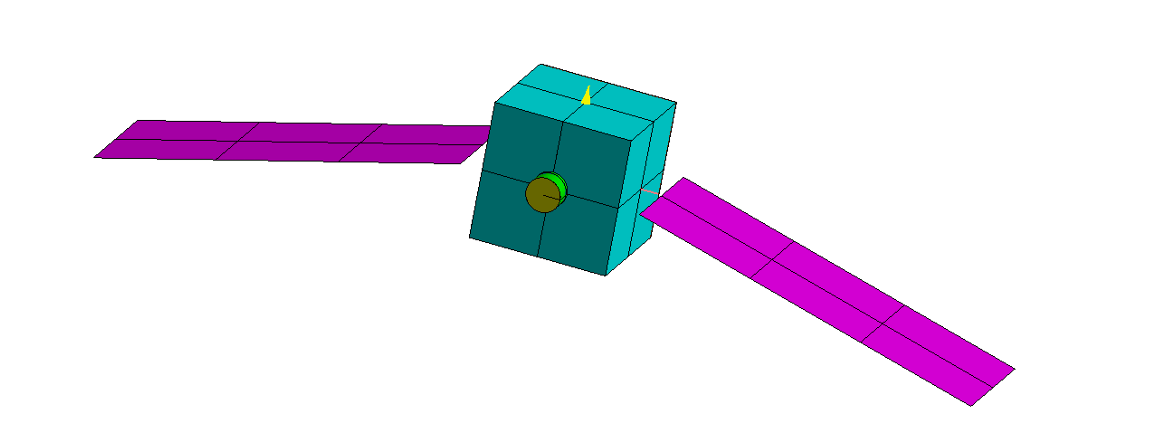
\includegraphics[width=\textwidth]{Figures/03/HELIOS.png}
        \caption{External view of the satellite model.}
        \label{fig:helios_external}
    \end{subfigure}

    \vspace{0.4cm}

    \begin{subfigure}[t]{0.9\textwidth}
        \centering
        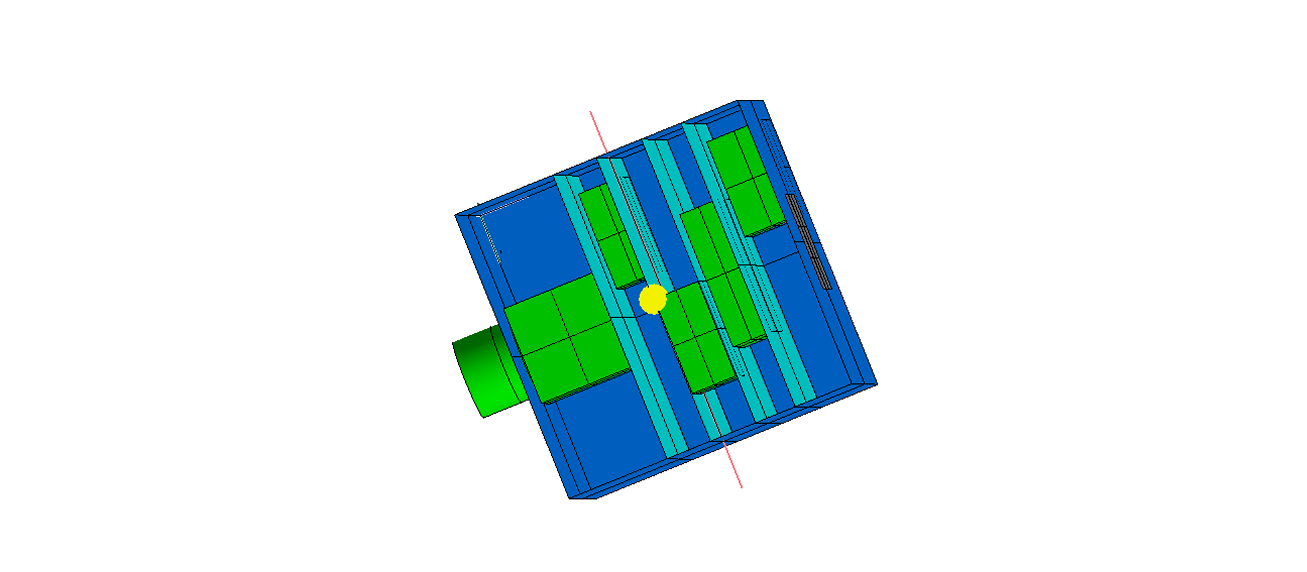
\includegraphics[width=\textwidth]{Figures/03/geom_HELIOS.png}
        \caption{Internal view of the satellite model.}
        \label{fig:helios_internal}
    \end{subfigure}

    \caption{External and internal views of the HELIOS thermal model. Taken
    from \cite{tfg_carol}.}
    \label{fig:helios_geometry}
\end{figure}

The steady-state solution of HELIOS contains the thermal data that are
extracted and organised by the initial Python code before being examined
through the graphical interface. The application developed for this thesis uses
a separate spacecraft thermal model with several cyclic transient analysis
cases.

\section{Python-Based Post-Processing of Steady-State Cases} 
\label{sec:previous_application} 

The initial Python-based implementation uses the steady-state results generated
for the HELIOS model in \acrshort{esatan-tms}~\cite{tfg_carol}. In this type
of analysis, a single temperature is calculated for each node under the
selected boundary conditions, while the corresponding thermal loads and heat
flows remain independent of time.

The imported results are linked to the hierarchy defined for the thermal
model, so that each node can be located within the corresponding component and
subsystem. Instead of working directly with the complete list of node
identifiers contained in the \acrshort{esatan-tms} files, the user can examine
the results through the spacecraft structure. This relationship between the
thermal data and the physical model helps identify the origin of each value and
interpret it in an engineering context.  

The main modules of this codebase and their connections are shown in
Figure~\ref{fig:helios_previous_architecture}.

\begin{figure}[H]
    \centering
    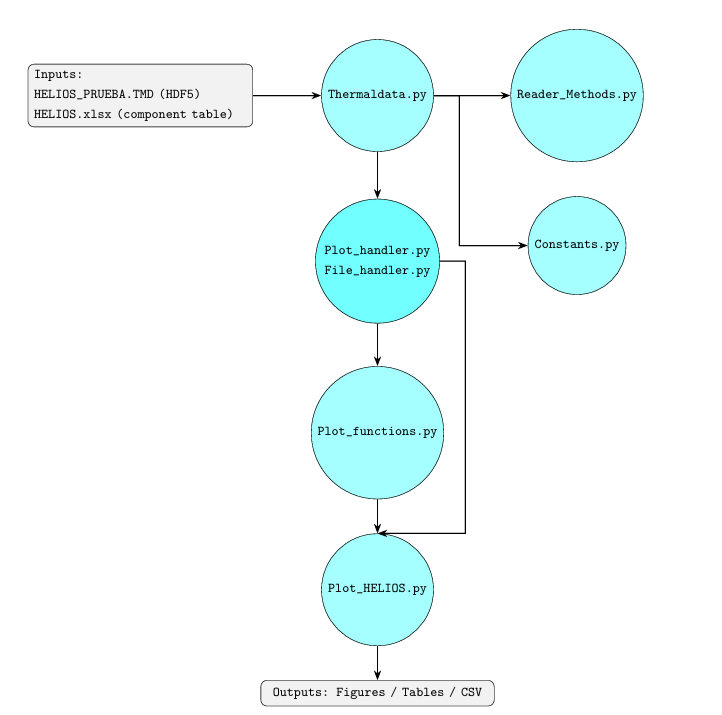
\includegraphics[width=0.78\textwidth]
    {Figures/03/arquitectura_HELIOS.png}
    \caption{Architecture of the initial post-processing implementation.
    Taken from \cite{tfg_carol}.}
    \label{fig:helios_previous_architecture}
\end{figure}

The architecture separates result reading, data organisation and 
representation. \texttt{Thermaldata.py} imports the HELIOS result file and 
the external component table, while the supporting modules handle data 
selection, file management and plotting. The interface is provided by 
\texttt{Plot\_HELIOS.py}, from which figures, tables and data files can be 
generated \cite{tfg_carol}.

This implementation is suitable for examining the thermal results of an individual
steady-state case. However, it does not provide complete post-processing of
transient results or allow several simulation cases to be loaded and compared
simultaneously. Extending the same structure to time-dependent results and
multiple cases requires changes to both data management and representation.

\section{Motivation for the Present Work}
\label{sec:project_motivation}

Transient simulations associate each calculated value with a specific
simulation time. The post-processing tools must preserve this correspondence
when results are selected, represented, and compared, particularly when
several components or interfaces are considered together.

During an orbital cycle, transitions between solar illumination and eclipse
and changes in internal dissipation produce variations in the thermal response
of the spacecraft. These variations must therefore be examined throughout the 
orbital cycle to determine when they occur and which elements are most affected.

Comparing simulation cases introduces an additional requirement. Spacecraft
thermal analyses may include several cases representing different
environmental and operating conditions. Processing them separately requires
equivalent elements to be selected again for every case and prevents their
direct comparison within the same representation. Managing cases associated
with the same thermal model together allows equivalent selections to be
applied and the differences between them to be calculated consistently.

For these reasons, the application is extended to process transient
results and manage several simulation cases associated with the same thermal
model. This allows equivalent components and interfaces to be compared
throughout the simulated period and the intervals in which the differences
between cases are most significant to be identified.